\documentclass[12pt, twoside]{article}
\input{../preamble}
\usepackage{float}

\title{Physics}
\author{Chris Huson}
\date{May 2026}

\fancyhead[LE]{\thepage}
\fancyhead[RO]{\thepage \\ First \& last name: \hspace{2.25cm} \,\\  \,}
\fancyhead[LO]{La Scuola d'Italia / Huson / Physics \\* 19 May 2026}

\begin{document}

\subsubsection*{3.5 Quiz: Vectors, Frames of Reference, and Energy}

\begin{enumerate}

\item \textbf{Matching: physicists and their work.} Each description below corresponds to one of the physicists listed. Write the letter of the matching description in the blank next to each name.

\vspace{0.3cm}

\begin{tabular}{rl}
Newton (1687) & \rule{2cm}{0.4pt} \\[0.5cm]
Michelson \& Morley (1887) & \rule{2cm}{0.4pt} \\[0.5cm]
Poincaré (1900) & \rule{2cm}{0.4pt} \\[0.5cm]
Lorentz (1904) & \rule{2cm}{0.4pt} \\[0.5cm]
Einstein (1905) & \rule{2cm}{0.4pt} \\
\end{tabular}

\vspace{0.6cm}

\begin{enumerate}[label=(\alph*), itemsep=0.4cm]
\item Used a sensitive interferometer to attempt to detect Earth's motion through the ``ether'' --- the supposed medium through which light was thought to propagate. The experiment produced a \emph{null result}: no measurable difference in the speed of light could be found, regardless of Earth's orbital motion.

\item Proposed that the speed of light is a constant when measured by observers in any inertial frame of reference, regardless of the motion of the source or the observer. This single postulate leads to profound implications for our understanding of space, time, mass, and energy --- including length contraction, time dilation, and the mass--energy equivalence $E = mc^{2}$.

\item His scientific theory of the laws of motion and universal gravitation were the predominant basis of physics until they were challenged by experimental results in the late 1800s.

\item Developed the transformation equations relating space and time coordinates measured by two observers in relative motion:
\[
x' = \gamma(x - vt), \qquad t' = \gamma\!\left(t - \dfrac{vx}{c^{2}}\right), \qquad \gamma = \dfrac{1}{\sqrt{1 - v^{2}/c^{2}}}
\]

\item Articulated the principle that the laws of physics should appear the same to all observers in uniform motion. Crucially, he argued that the \emph{simultaneity} of distant events is not absolute --- whether two events at separate locations happen ``at the same time'' depends on the observer's frame of reference, since clocks at different places must be synchronized using light signals. His work helped develop the mathematical framework that anticipated key ideas of relativity.
\end{enumerate}

\newpage

\item \textbf{Effects on measurements at high relative speed.} Briefly describe what an observer measures for an object moving at a large fraction of the speed of light relative to that observer. Address each of the following:
\vspace{0.3cm}
\begin{enumerate}[itemsep=4.5cm]
\item Length of the object in the direction of relative motion.
\item Measurement of elapsed time (e.g., the rate of a moving clock).
\item Inertia of the object --- that is, the force required to increase its velocity (sometimes phrased as the object's ``effective mass'').
\vspace{2cm}
\end{enumerate}

\newpage

\item A force $\vec{F}$ of magnitude $100\,\text{N}$ is directed at $53^\circ$ above the horizontal, as shown.\vspace{0.25cm}
\begin{multicols}{2}
  \begin{enumerate}[itemsep=5cm]
    \item Find the horizontal component $F_x$.
    \item Find the vertical component $F_y$.\vspace{4cm}
  \end{enumerate}
  \begin{flushright}
    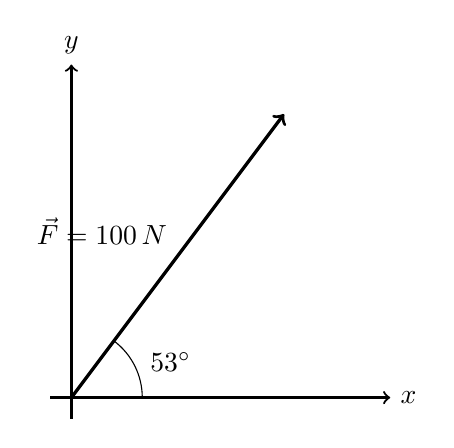
\begin{tikzpicture}[scale=0.9]
      \draw[->, thick] (-0.3,0)--(4.5,0) node[right]{$x$};
      \draw[->, thick] (0,-0.3)--(0,4.7) node[above]{$y$};
      \draw[->, very thick] (0,0)--(3,4) node[midway, above left]{$\vec{F}=100\,\text{N}$};
      \draw (1,0) arc [start angle=0, end angle=53, radius=1];
      \node at (1.4,0.5){$53^\circ$};
    \end{tikzpicture}
  \end{flushright}
\end{multicols}

\newpage

\item A car's velocity has components $v_x = 8\,\text{m/s}$ (east) and $v_y = 6\,\text{m/s}$ (north).\vspace{0.25cm}
\begin{multicols}{2}
  \begin{enumerate}[itemsep=4cm]
    \item Find the speed $|\vec{v}|$.
    \item Find the direction $\theta$, measured north of east, to the \emph{nearest degree}.\vspace{4cm}
  \end{enumerate}
  \begin{flushright}
    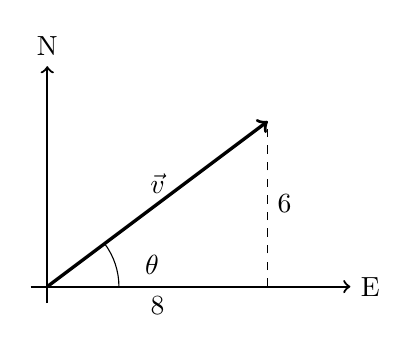
\begin{tikzpicture}[scale=0.7]
      \draw[->, thick] (-0.3,0)--(5.5,0) node[right]{E};
      \draw[->, thick] (0,-0.3)--(0,4) node[above]{N};
      \draw[->, very thick] (0,0)--(4,3) node[midway, above]{$\vec{v}$};
      \draw[dashed] (4,0)--(4,3);
      \node at (4,1.5)[right]{$6$};
      \node at (2,0)[below]{$8$};
      \draw (1.3,0) arc [start angle=0, end angle=36.87, radius=1.3];
      \node at (1.9,0.4){$\theta$};
    \end{tikzpicture}
  \end{flushright}
\end{multicols}

\vspace{4cm}

\item \textbf{Frame of reference --- on a train.} A train travels east at $30\,\text{m/s}$ relative to the ground. A passenger walks toward the front of the train at $2.0\,\text{m/s}$ relative to the train.
  \begin{enumerate}[itemsep=4cm]
    \item What is the passenger's velocity relative to the ground?
    \item A car drives \emph{west} at $20\,\text{m/s}$ relative to the ground. What is the passenger's velocity relative to the car? That is, what is the train passenger's relative velocity as measured by an observer in the car?
    \vspace{2cm}
  \end{enumerate}

\newpage

\item \textbf{Frame of reference --- airplane in wind.} A small plane heads due east at $60\,\text{m/s}$ relative to the air. A steady wind blows from south to north at $25\,\text{m/s}$ relative to the ground.\vspace{0.25cm}
\begin{multicols}{2}
  \begin{enumerate}[itemsep=5cm]
    \item Find the plane's speed relative to the ground.
    \item Find the angle of the plane's motion, measured north of east, to the \emph{nearest degree}.\vspace{4cm}
  \end{enumerate}
  \begin{flushright}
    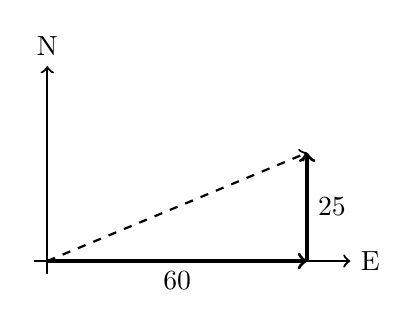
\begin{tikzpicture}[scale=0.55]
      \draw[->, thick] (-0.3,0)--(7,0) node[right]{E};
      \draw[->, thick] (0,-0.3)--(0,4.5) node[above]{N};
      \draw[->, very thick] (0,0)--(6,0) node[midway, below]{$60$};
      \draw[->, very thick] (6,0)--(6,2.5) node[midway, right]{$25$};
      \draw[->, thick, dashed] (0,0)--(6,2.5);
    \end{tikzpicture}
  \end{flushright}
\end{multicols}

\newpage

\item \textbf{Energy unit conversions.} A medium banana contains about $4.0\times 10^{5}\,\text{J}$ of chemical energy available when metabolized.
  \begin{enumerate}[itemsep=5cm]
    \item Convert this to kilocalories. ($1\,\text{kcal} = 4184\,\text{J}$.)
    \item Convert this to kilowatt-hours. ($1\,\text{kWh} = 3.6\times 10^{6}\,\text{J}$.)
    \item How many electron-volts is $4.0\times 10^{5}\,\text{J}$? ($1\,\text{eV} = 1.6\times 10^{-19}\,\text{J}$.)
  \end{enumerate}

\end{enumerate}
\end{document}
